\documentclass[tikz,border=2pt]{standalone}
\usepackage{amsmath}
\usepackage{pgfplots}
\pgfplotsset{compat=1.18}
\usetikzlibrary{arrows.meta}
\begin{document}
% Prisoner's dilemma (3,3),(0,5),(5,0),(1,1): average discounted payoff of the stream 3,3,3,...
% is 3; of the one-time defection stream 5,1,1,... it is 5 - 4 delta. They cross at
% delta = 1/2 = (5-3)/(5-1); at delta = 0.9 the values are 3 and 1.4.
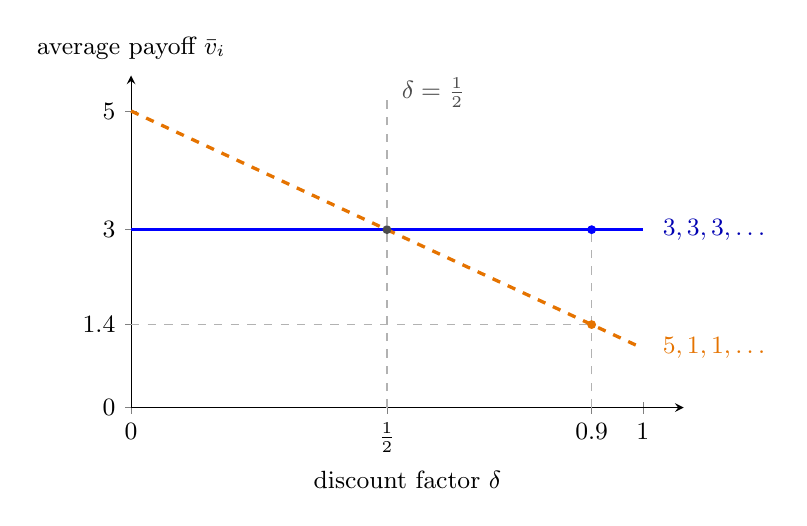
\begin{tikzpicture}[font=\small, >={Latex[length=2mm]}]
  \begin{axis}[
    axis lines=left, xmin=0, xmax=1.08, ymin=0, ymax=5.6,
    xtick={0,0.5,0.9,1}, ytick={0,1.4,3,5},
    xticklabels={$0$,$\tfrac12$,$0.9$,$1$}, yticklabels={$0$,$1.4$,$3$,$5$},
    xlabel={discount factor $\delta$}, ylabel={average payoff $\bar v_i$},
    ylabel style={rotate=-90, anchor=south, at={(axis description cs:0,1.02)}},
    width=8.6cm, height=5.8cm, clip=false]
    \addplot[gray!60, thick, dashed] coordinates {(0.5,0) (0.5,5.3)};
    \addplot[gray!60, thin, dashed] coordinates {(0.9,0) (0.9,3)};
    \addplot[gray!60, thin, dashed] coordinates {(0,1.4) (0.9,1.4)};
    \addplot[blue, very thick, domain=0:1, samples=2] {3};
    \addplot[orange!90!black, very thick, dashed, domain=0:1, samples=2] {5-4*x};
    \fill[blue] (axis cs:0.9,3) circle (1.6pt);
    \fill[orange!90!black] (axis cs:0.9,1.4) circle (1.6pt);
    \fill[gray!60!black] (axis cs:0.5,3) circle (1.6pt);
    \node[blue!70!black, anchor=west] at (axis cs:1.02,3) {$3,3,3,\dots$};
    \node[orange!90!black, anchor=west] at (axis cs:1.02,1) {$5,1,1,\dots$};
    \node[gray!60!black, anchor=south west] at (axis cs:0.51,4.9) {$\delta=\tfrac12$};
  \end{axis}
\end{tikzpicture}
\end{document}
